\section*{Part 1. Solution of ODE-systems with constant coefficients}

Starting from the described electrical circuit, we get the differential equation
$$L\ddot{q}+R\dot{q}+\frac{1}{C}q = E,\hspace*{5mm}q(0)=0,\hspace*{5mm}\dot{q}(0)=0,$$
after defining the variable $\dot{q}=i$. We easily rewrite this as a first order system of linear equations. Setting $$\textbf{y}= \begin{pmatrix}
y(1)\\
y(2)\\
\end{pmatrix} = \begin{pmatrix}
q\\
\dot{q}\\
\end{pmatrix},$$
this gives
%$$ \left.\begin{array}{lll}
%\dot{y}(1) & = & y(2)\\
%\dot{y}(2) & = & -\frac{R}{L}y(2) - \frac{1}{LC}y(1) + %\frac{E}{L}
%\end{array}\right. $$
$$\begin{pmatrix}
\dot{y}(1)\\
\dot{y}(2)\\
\end{pmatrix}= \begin{pmatrix}
0 & 1\\
- \frac{1}{LC} & -\frac{R}{L}\\
\end{pmatrix}\begin{pmatrix}
y(1)\\
y(2)\\
\end{pmatrix}
+ \begin{pmatrix}
0\\
E\\
\end{pmatrix}.$$
Lets define the matrix 
$$A=\begin{pmatrix}
0 & 1\\
- \frac{1}{LC} & -\frac{R}{L}\\
\end{pmatrix}$$ for some parameters $R$, $L$, $C$.

This problem is linear and the stability analysis of the problem is therefore quite straightforward. The problem will be stable if the real part of all the eigenvalues of A are negatives. Assume any combination of $R$, $L$, $C$ that are all positives, we have $\det(A)= \lambda_1 \lambda_2 = \dfrac{1}{LC}>0$ and $\text{trace}(A)= \lambda_1 + \lambda_2 = -\frac{R}{L}<0$. This clearly ensures that all eigenvalues are negative and guaranties stability.

Below is our Matlab code for this question. The chosen value of $E$ was 1 because we can see in the analytical solution that it is just a scaling factor.


The solution of the equation is shown on figure \ref{result1} for al the values of R. As we saw, the system is stable for all positive values of $R,L,C$. For small values of $R$, we can see that the system is oscillating with decreasing amplitude. As $R$ increases, the system reaches the equilibrium faster. We can note that for $R=10$, the system behaves like an RC-system. This happens because the inductance becomes neglectable due to the small current.

\begin{figure}
\begin{center}
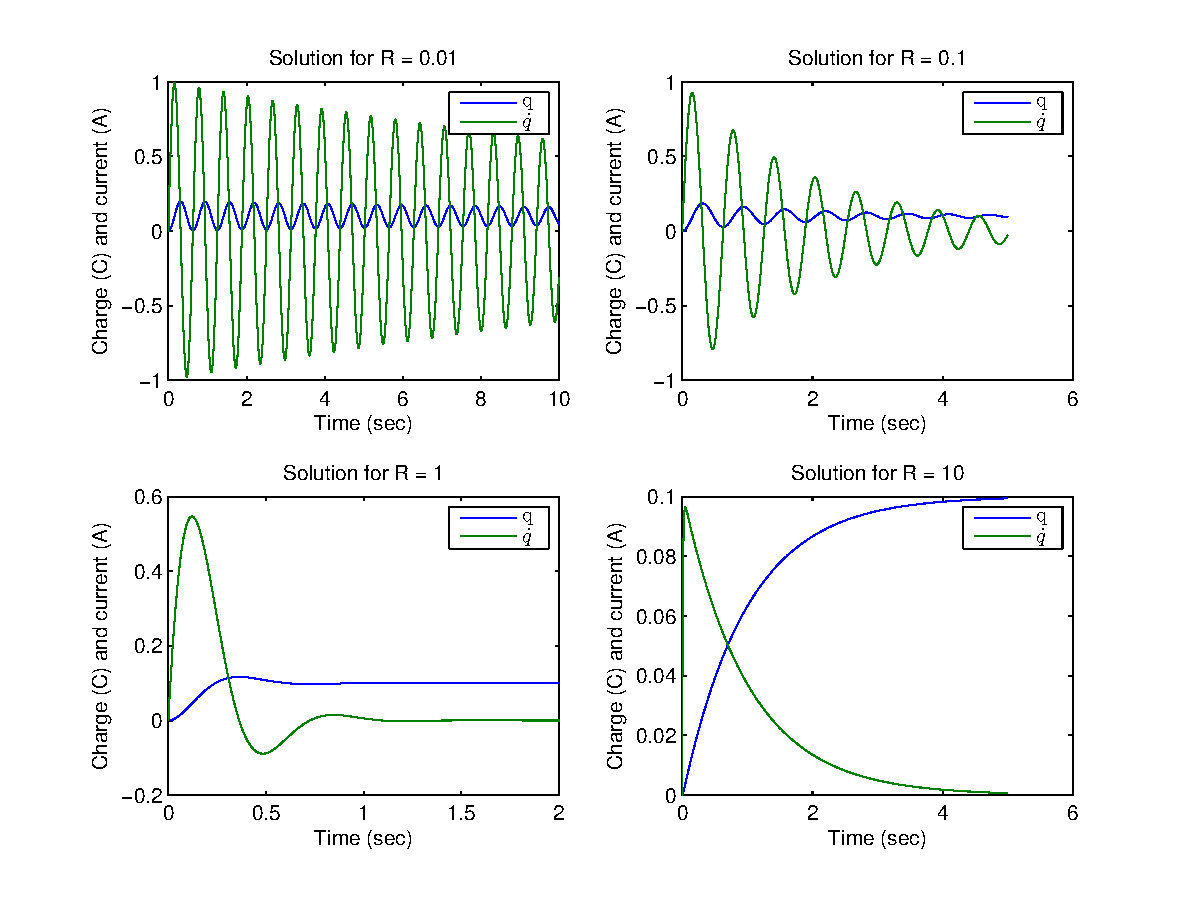
\includegraphics[scale=0.5]{result1.eps}
\caption{Solutions of the system in part 1 for various values of R}
\label{result1}
\end{center}
\end{figure}
 
\FloatBarrier 
 
\lstinputlisting{LAB1_1.m}% for a file
